\documentclass[11pt,a4paper]{article}
\usepackage[utf8]{inputenc}
\usepackage[T1]{fontenc}
\usepackage[french]{babel}
\usepackage{lmodern,microtype}
\usepackage[margin=2.1cm]{geometry}
\usepackage{amsmath,booktabs,graphicx,xcolor,hyperref}
\definecolor{blueNG}{HTML}{174A70}
\hypersetup{colorlinks=true,linkcolor=blueNG,urlcolor=blueNG}
\graphicspath{{figures/}}
\title{\textcolor{blueNG}{Supplément expérimental : discrimination de chiffres manuscrits}\\[.25em]\large Sonde adaptative, neurones de référence et composition en 64 dimensions}
\author{Dossier expérimental NGeGenBrain}
\date{28 octobre 2026}
\begin{document}\maketitle
\begin{abstract}
Ce supplément élargit l'évaluation réelle au benchmark de chiffres manuscrits 8×8 de scikit-learn, filtré sur les chiffres 3 et 8. L'entrée comporte 64 intensités de pixels. Les quatre méthodes de classification sont comparées sur les mêmes partitions et les sondes remplacent ensuite des unités cachées d'un MLP enseignant. Cette expérience supplémentaire n'appartient pas au protocole primaire v1.1 ; son protocole propre a été haché avant son exécution. Elle constitue un benchmark réel de classification, et non un déploiement opérationnel.
\end{abstract}

\section{Question et données}
Le but est d'augmenter la difficulté d'entrée par rapport aux tâches synthétiques à deux dimensions et au benchmark de diagnostic de 30 variables. Le dataset \texttt{load\_digits} contient des images matricielles 8×8 ; seuls les exemples dont l'étiquette originale est 3 ou 8 sont conservés. Le chiffre 3 devient la classe 0, le chiffre 8 la classe 1. Le jeu filtré contient 357 exemples et 64 caractéristiques.

\section{Protocole gelé}
Les graines sont 714, 825 et 936. Pour chacune, le split stratifié suit train/validation/test environ 60/20/20 (213/72/72 exemples par graine), et le standardiseur est ajusté exclusivement sur train. Les méthodes A (RBF adaptative), B (RBF avec taux par groupe méta-appris), le contrôle RBF fixe et le MLP à 16 unités sont comparés sur les mêmes exemples de test. B utilise 35 étapes de méta-ajustement train/validation et 700 époques finales ; les autres méthodes utilisent 220 époques finales. Le test n'est pas un argument des fonctions d'ajustement.

La composition utilise un MLP enseignant à 16 unités cachées, appris sur train seul. Les sondes scalaires RBF imitent les activations des neurones à partir d'observations d'entrées/activations train ; on remplace 1, 4 puis 16 unités. La lecture de sortie de l'enseignant est conservée. Chaque neurone enseignant sur entrée 64D a 65 paramètres (64 poids et un biais), alors qu'une sonde RBF scalaire à 8 centres a 529 paramètres entraînables. Ce déséquilibre est déclaré et interdit d'interpréter la comparaison comme une égalité de capacité.

Le protocole v1.0 et le correctif administratif v1.0.1, ainsi que leurs empreintes, sont fournis séparément. Le premier lancement avait terminé les calculs mais échoué à sérialiser le rapport d'audit ; après correction du seul sérialiseur, les CSV de prédictions, classification, composition et fidélité ont été reproduits octet par octet.

\section{Classification comparative}
Les valeurs sont les moyennes et écarts-types de l'exactitude, F1 et ROC-AUC sur trois graines indépendantes. Ces écarts-types sont descriptifs ; n=3 ne permet pas de conclure à une supériorité universelle.
\begin{table}[htbp]\centering\small
\begin{tabular}{lrrrrr}\toprule
Méthode & Paramètres & Exactitude (\%) & F1 (\%) & ROC-AUC & Log-loss \\\midrule
RBF fixe & 17 & 91.20 $\pm$ 4.47 & 91.35 $\pm$ 4.29 & 0.9727 $\pm$ 0.0183 & 0.3516 $\pm$ 0.0301 \\
RBF adaptative A & 1057 & 95.37 $\pm$ 2.89 & 95.40 $\pm$ 2.84 & 0.9951 $\pm$ 0.0047 & 0.1521 $\pm$ 0.0320 \\
Mécanisme appris B & 1057 & 96.76 $\pm$ 2.12 & 96.73 $\pm$ 2.11 & 0.9979 $\pm$ 0.0019 & 0.0827 $\pm$ 0.0234 \\
MLP référence & 1057 & 99.07 $\pm$ 1.60 & 99.07 $\pm$ 1.60 & 1.0000 $\pm$ 0.0000 & 0.0216 $\pm$ 0.0207 \\\bottomrule\end{tabular}
\caption{Classification binaire des chiffres 3 et 8. Moyenne $\pm$ écart-type sur trois splits. Les sondes RBF adaptative et le MLP possèdent le même nombre de paramètres ; le contrôle fixe est beaucoup plus petit.}\end{table}

\begin{figure}[htbp]\centering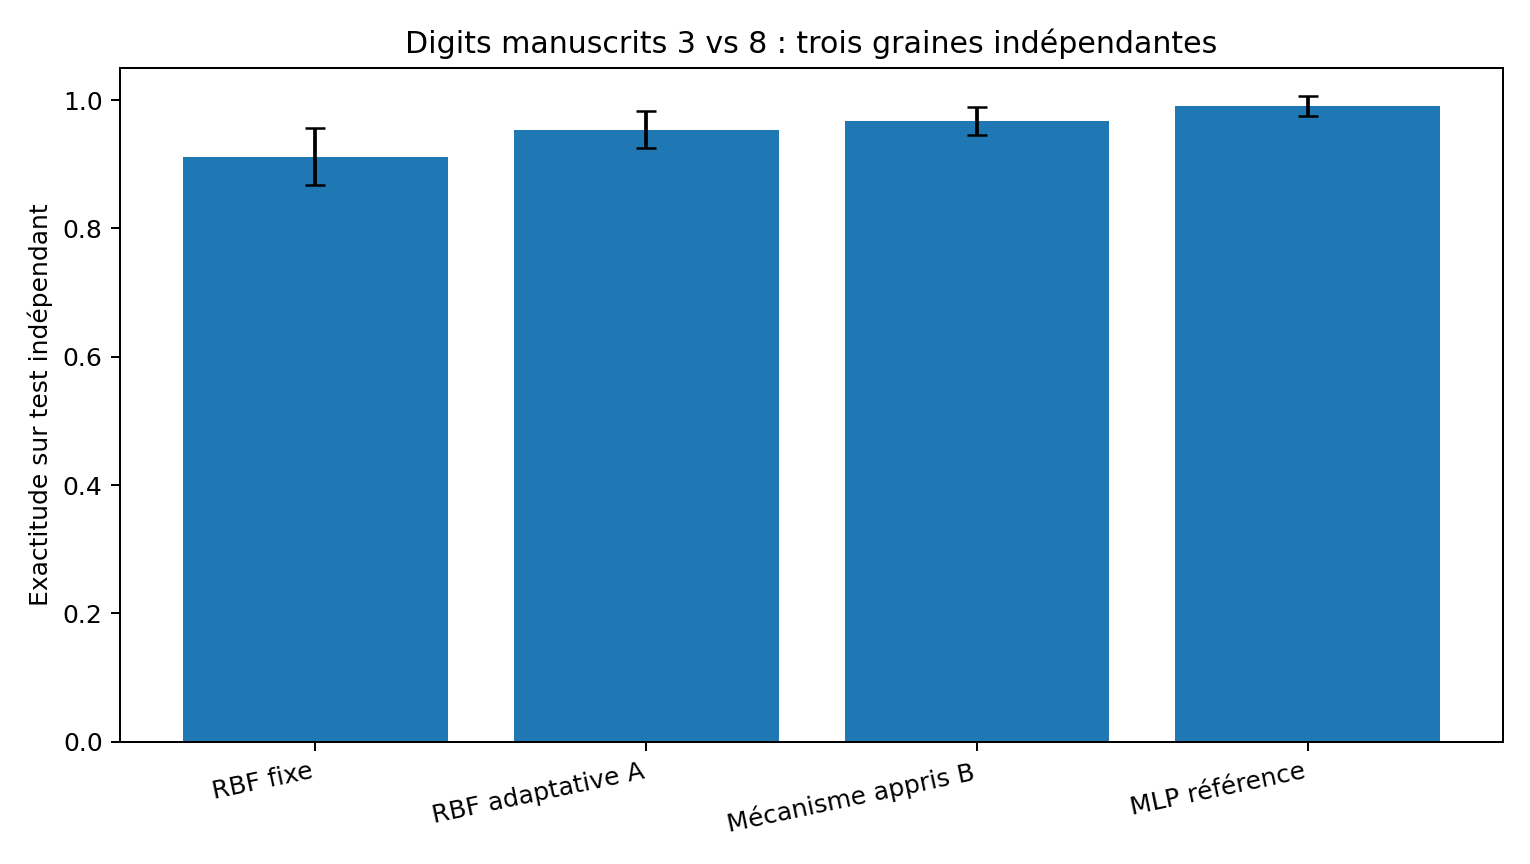
\includegraphics[width=.82\textwidth]{digits_3_vs_8_comparison_exploratoire.png}\caption{Exactitude sur le test gelé.}\end{figure}

Le MLP obtient le meilleur score moyen. B est compétitive (96.76\%) mais ne dépasse pas le MLP (99.07\%). Le contrôle fixe est moins performant, mais il n'a que 17 paramètres contre 1057 ; il ne permet pas d'isoler l'effet de l'adaptation du seul effet de capacité.

\section{Composition et remplacement}
\begin{table}[htbp]\centering\small
\begin{tabular}{rrrr}\toprule
Unités remplacées & Exactitude enseignant (\%) & Exactitude après (\%) & Écart logits absolu \\\midrule
1 & 98.15 $\pm$ 3.21 & 98.15 $\pm$ 3.21 & 0.122 $\pm$ 0.027 \\
4 & 98.15 $\pm$ 3.21 & 97.22 $\pm$ 2.41 & 0.494 $\pm$ 0.001 \\
16 & 98.15 $\pm$ 3.21 & 95.83 $\pm$ 0.00 & 1.969 $\pm$ 0.081 \\\bottomrule\end{tabular}
\caption{Composition après remplacement de sondes. Moyenne $\pm$ écart-type sur trois graines.}\end{table}

\begin{figure}[htbp]\centering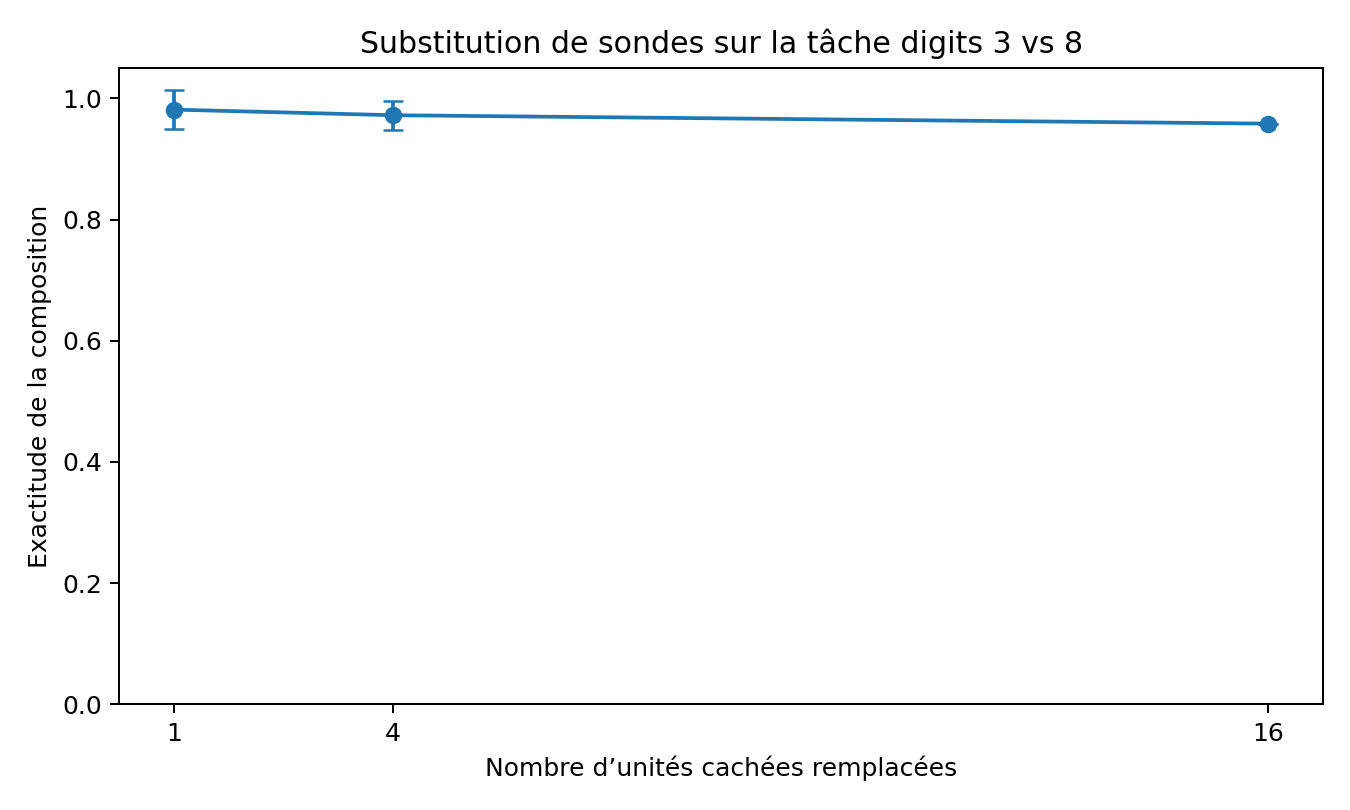
\includegraphics[width=.72\textwidth]{digits_3_vs_8_composition_accuracy_exploratoire.png}\caption{Exactitude de la composition selon le nombre d'unités remplacées.}\end{figure}
\begin{figure}[htbp]\centering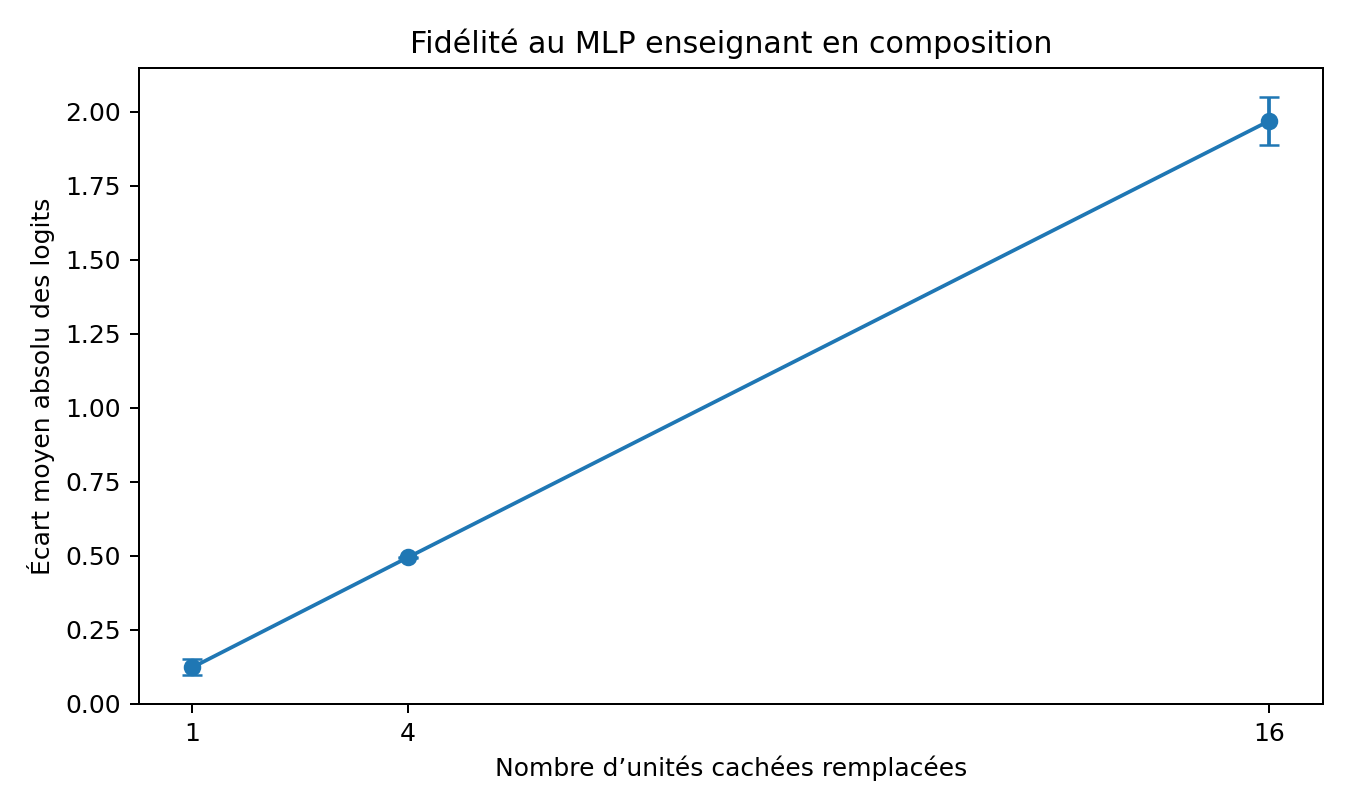
\includegraphics[width=.72\textwidth]{digits_3_vs_8_composition_logit_delta_exploratoire.png}\caption{Déviation moyenne des logits par rapport au MLP enseignant.}\end{figure}

L'erreur moyenne sur les activations cachées est MAE $0.2599\pm0.0089$, RMSE $0.3301\pm0.0237$ et $R^2=0.8677\pm0.0201$ après moyenne des 16 unités dans chaque graine puis agrégation des trois graines. La fidélité diminue à mesure qu'on remplace davantage d'unités : l'écart des logits atteint environ 1.969 quand toutes les unités sont substituées. La stabilité partielle de l'exactitude ne signifie donc pas que le comportement numérique du réseau enseignant a été reproduit.

\section{Audit et limites}
Le registre d'audit contient 357 exemples par graine et zéro chevauchement des empreintes de lignes entre train, validation et test. Les tailles de classes sont identiques par split dans chacune des graines : train 109/104, validation 37/35, test 37/35 pour les classes 3/8. Le test intervient seulement après gel des modèles. Les empreintes SHA-256 des CSV du premier calcul et de la relance après correction du sérialiseur sont identiques.

Limites : (1) il s'agit de la tâche binaire 3-vs-8, pas de la classification des dix chiffres ; (2) le dataset est petit et le test ne remplace pas une validation d'usage ; (3) les sondes de composition utilisent beaucoup plus de paramètres que chaque neurone source ; (4) la sortie aval du MLP enseignant est conservée ; (5) trois graines donnent une base statistique limitée ; (6) les résultats représentent une extension exploratoire préenregistrée séparément, non une partie du protocole primaire v1.1.

\section{Conclusion}
Sur ce benchmark réel à 64 caractéristiques, la sonde adaptative apprend correctement la tâche mais reste en moyenne en dessous du MLP de référence ; le méta-apprentissage des taux réduit la perte et améliore le score par rapport à A dans ces essais, sans dépasser le MLP. L'imitation des activations cachées devient sensiblement moins fidèle après remplacement de nombreux neurones. Ces résultats sont compatibles avec une approximation fonctionnelle sous budget donné, mais ne démontrent pas une équivalence générale entre sonde et neurone.
\end{document}
